\documentclass[12pt]{exam}
\usepackage[homework,id=3]{cs161}
\usepackage{graphicx}
\usepackage{listings}
\usepackage{pdfpages}
\usepackage{seqsplit}

\usepackage{array}
\usepackage{hyperref}
\usepackage{subfiles}
\usepackage{etoolbox}

\lstset{
language=C,                % choose the language of the code
basicstyle=\scriptsize,       % the size of the fonts that are used for the code
numbers=left,                   % where to put the line-numbers
numberstyle=\scriptsize,      % the size of the fonts that are used for the line-numbers
stepnumber=1,                   % the step between two line-numbers. If it is 1 each line will be numbered
numbersep=5pt,                  % how far the line-numbers are from the code
backgroundcolor=\color{white},  % choose the background color. You must add \usepackage{color}
showspaces=false,               % show spaces adding particular underscores
showstringspaces=false,         % underline spaces within strings
showtabs=false,                 % show tabs within strings adding particular underscores
frame=single,           % adds a frame around the code
tabsize=2,          % sets default tabsize to 2 spaces
captionpos=b,           % sets the caption-position to bottom
breaklines=true,        % sets automatic line breaking
breakatwhitespace=false,    % sets if automatic breaks should only happen at whitespace
escapeinside={\%*}{*)}          % if you want to add a comment within your code
}

\newcommand{\solbox}[2]{%
\fbox{%
\parbox[c][#1][t]{\dimexpr\linewidth-2\fboxsep-2\fboxrule}{
  \hrule width \hsize height 0pt
  #2
 }%
}%
\par\vspace{\ht\strutbox}
}
\makeatother

\usepackage{etoolbox}
\newtoggle{pdfform}
\togglefalse{pdfform} % may be toggled true in configuration

\InputIfFileExists{config}{}

\newcommand{\textfield}[3]{%
\iftoggle{pdfform}{%
\TextField[name = #1, backgroundcolor=white, height=#2,
width = \linewidth, multiline=true]{\mbox}%
}{%
\ifprintanswers\else{%
    \solbox{#2}{#3}}
\fi%
}%
}

\newcommand{\includesolution}[1]{%
\IfFileExists{solutions/#1.tex}{%
\begin{solution}%
\subfile{solutions/#1.tex}%
\end{solution}%
}{}
}



\newcommand{\checkbox}[3]{%
\iftoggle{pdfform}{%
\CheckBox[name = #1, backgroundcolor=white, bordercolor=black, #2]{}%
}{%
\ifprintanswers\else%
\framebox[0.6cm]{\rule{0pt}{0.4cm}#3}
\fi%
}%
}

\def\duedate{Friday, 22 March 2019}

\begin{document}
\begin{Form}

\begin{center}
  \large
  Due: \duedate, at 11:59pm
\end{center}

\paragraph{Instructions.}
This homework is due \textbf{\duedate, at 11:59pm}. 

\bigskip

You may use any of the following methods to complete your homework:
\begin{itemize}
    \item Use the LaTeX template provided on Piazza to fill out your responses; or
    \item Use Adobe Acrobat to fill in this fillable PDF; or
    \item Print this paper out and handwrite your solutions, but \textbf{please make sure your responses do not overflow the box provided} before submitting to ensure that you get full credit for your response.
\end{itemize}
  

\textbf{}

\begin{questions}

\newpage

\titledquestion{TLS}[20]

Alice wants to communicate with \texttt{smallfish.com} using TLS. 
Assume the browser and server use RSA-based key exchange (not Diffie-Hellman).
Each part is independent. 
 Assume that the cipher-suites chosen in the TLS connections \textbf{do not} make use of TLS sequence numbers. Assume each potential replay attack involves generating a new TLS connection.

\begin{parts}
\part Suppose Alice downloads a buggy version of the Firefox browser
that implements TLS incorrectly.
The TLS specification says that, during the handshake, the
browser should send a random 256-bit number $R_B$ and the server should send
a random 256-bit number $R_S$.\footnote{Also recall Discussion 7, Q2 here:
\href{https://inst.eecs.berkeley.edu/~cs161/sp19/sections/07.pdf}{https://inst.eecs.berkeley.edu/\textasciitilde{}cs161/sp19/sections/07.pdf}}
Instead of picking $R_B$ randomly, it increments a counter and
sends it instead.
Which of the following are true? \textbf{Select all that apply}.

\checkbox{Q1P1O1Y}{width=1.5em}{
%Yes/No directions: uncomment 'X' to make it appear
X
} 
If Alice visits a HTTPS URL, a man-in-the-middle can not
replay that HTTP request to the server a second time.

\checkbox{Q1P1O2Y}{width=1.5em}{
%Yes/No directions: uncomment 'X' to make it appear
%X
} 
If Alice visits the same HTTPS URL twice,
when Alice visits that URL the second time, a man-in-the-middle can
not replay the HTML page that was returned by the server
on Alice's first visit.

\checkbox{Q1P1O3Y}{width=1.5em}{
%Yes/No directions: uncomment 'X' to make it appear
%X
} 
A man-in-the-middle can not compromise Alice's confidentiality
(e.g., learn the data she sends over TLS).

\checkbox{Q1P1O4Y}{width=1.5em}{
%Yes/No directions: uncomment 'X' to make it appear
%X
} 
A man-in-the-middle can not learn the symmetric MAC keys that protect
data sent over TLS connections initiated by Alice's browser.

\checkbox{Q1P1O5Y}{width=1.5em}{
%Yes/No directions: uncomment 'X' to make it appear
%X
} 
None of the above

\bigskip

\newpage
\part Alice downloads a patch for her buggy version of Firefox, which fixes the
previous problem but introduces another bug. Now, her client generates the
pre-master secret based on three items: the current absolute time, the total
time Alice's computer has been powered on, and the process-ID of the current
Firefox process. Which of the following are true? \textbf{Select all that apply}.

\checkbox{Q1P2O1Y}{width=1.5em}{
%Yes/No directions: uncomment 'X' to make it appear
%X
} 
If Alice visits a HTTPS URL, a man-in-the-middle can not
replay that HTTP request to the server a second time.

\checkbox{Q1P2O2Y}{width=1.5em}{
%Yes/No directions: uncomment 'X' to make it appear
%X
} 
If Alice visits the same HTTPS URL twice,
when Alice visits that URL the second time a man-in-the-middle can
not replay the HTML page that was returned by the server
on Alice's first visit.

\checkbox{Q1P2O3Y}{width=1.5em}{
%Yes/No directions: uncomment 'X' to make it appear
%X
} 
A man-in-the-middle can not compromise Alice's confidentiality
(e.g., learn the data she sends over TLS).

\checkbox{Q1P2O4Y}{width=1.5em}{
%Yes/No directions: uncomment 'X' to make it appear
%X
} 
A man-in-the-middle can not learn the symmetric MAC keys that protect
data sent over TLS connections initiated by Alice's browser.

\checkbox{Q1P2O5Y}{width=1.5em}{
%Yes/No directions: uncomment 'X' to make it appear
%X
} 
None of the above

\bigskip

\part Alice downloads an updated version of Firefox that is finally correct.
With her fixed browser, she visits \texttt{https://bluefish.com/}.
That server's TLS implementation has a bug: instead of picking
$R_S$ randomly, it always sends all zeros.
Which of the following are true? \textbf{Select all that apply}.

\checkbox{Q1P3O1Y}{width=1.5em}{
%Yes/No directions: uncomment 'X' to make it appear
%X
} 
If Alice visits a HTTPS URL, a man-in-the-middle can not
replay that HTTP request to the server a second time.

\checkbox{Q1P3O2Y}{width=1.5em}{
%Yes/No directions: uncomment 'X' to make it appear
%X
} 
If Alice visits the same HTTPS URL twice,
when Alice visits that URL the second time a man-in-the-middle can
not replay the HTML page that was returned by the server
on Alice's first visit.

\checkbox{Q1P3O3Y}{width=1.5em}{
%Yes/No directions: uncomment 'X' to make it appear
%X
} 
A man-in-the-middle can not compromise Alice's confidentiality
(e.g., learn the data she sends over TLS).

\checkbox{Q1P3O4Y}{width=1.5em}{
%Yes/No directions: uncomment 'X' to make it appear
%X
} 
A man-in-the-middle can not learn the symmetric MAC keys that protect
data sent over TLS connections initiated by Alice's browser.

\checkbox{Q1P3O5Y}{width=1.5em}{
%Yes/No directions: uncomment 'X' to make it appear
%X
} 
None of the above

\end{parts}


\newpage
\titledquestion{TCP}[10] 

Aisling has just opened her laptop and is attempting to connect to the Internet to visit \texttt{www.randomkittengenerator.com}.

Aoife, who works for the local Three-Letter Agency (TLA), is determined to interfere with Aisling's connection. The TLA (and, thus, Aoife) can leverage off-path, on-path, and man-in-the-middle attacks against Aisling, but they would prefer to use the easiest attack.
Recall that a man-in-the-middle can both observe as well as intercept traffic; an on-path attacker can observe traffic but not intercept it; and an off-path attacker can neither observe nor intercept traffic.
Hence, an off-path attack is easier to launch than on-path, and on-path is easier to launch than man-in-the-middle. 

For each scenario, which attack will Aoife use (on-path, off-path, or man-in-the-middle)?
\begin{parts}
    
    \part Aoife seeks to create a UDP request to the website's server which appears to come from Aisling's IP address. Aoife doesn't need to see the reply.
    
    \checkbox{Q2P1O1Y}{width=1.5em}{
    %Yes/No directions: uncomment 'X' to make it appear
    X
    } 
    Off-path
    
    
    \checkbox{Q2P1O2Y}{width=1.5em}{
    %Yes/No directions: uncomment 'X' to make it appear
    %X
    } 
    On-path
    
    \checkbox{Q2P1O3Y}{width=1.5em}{
    %Yes/No directions: uncomment 'X' to make it appear
    %X
    } 
    Man-in-the-middle

    
    \part Aoife seeks to create a TCP connection to the website's server which appears to be from Aisling's IP address. The server uses the current time to generate the initial sequence number. Aoife doesn't need to see the reply.
    
    \checkbox{Q2P2O1Y}{width=1.5em}{
    %Yes/No directions: uncomment 'X' to make it appear
    X
    } 
    Off-path
    
    
    \checkbox{Q2P2O2Y}{width=1.5em}{
    %Yes/No directions: uncomment 'X' to make it appear
    %X
    } 
    On-path
    
    \checkbox{Q2P2O3Y}{width=1.5em}{
    %Yes/No directions: uncomment 'X' to make it appear
    %X
    } 
    Man-in-the-middle
    
    \part Aoife seeks to create a TCP connection to the website's server which appears to be from Aisling's IP address. The server uses a secure RNG to generate the initial sequence number. Aoife doesn't need to see the reply.
    
    \checkbox{Q2P3O1Y}{width=1.5em}{
    %Yes/No directions: uncomment 'X' to make it appear
    %X
    } 
    Off-path
    
    
    \checkbox{Q2P3O2Y}{width=1.5em}{
    %Yes/No directions: uncomment 'X' to make it appear
    X
    } 
    On-path
    
    \checkbox{Q2P3O3Y}{width=1.5em}{
    %Yes/No directions: uncomment 'X' to make it appear
    %X
    } 
    Man-in-the-middle
    
    \newpage
    \part Aoife seeks to inject content into an existing active TCP connection between Aisling and the web server. Aoife knows Aisling is paranoid and records her raw traffic, but Aoife does not want Aisling to determine that Aoife has modified the traffic.
    
    \checkbox{Q2P4O1Y}{width=1.5em}{
    %Yes/No directions: uncomment 'X' to make it appear
    %X
    } 
    Off-path
    
    
    \checkbox{Q2P4O2Y}{width=1.5em}{
    %Yes/No directions: uncomment 'X' to make it appear
    %X
    } 
    On-path
    
    \checkbox{Q2P4O3Y}{width=1.5em}{
    %Yes/No directions: uncomment 'X' to make it appear
    X
    } 
    Man-in-the-middle
    
\end{parts}


\newpage
\titledquestion{DNS}[20] 

Okoro is a hacker attempting to sabotage CS161 from a cafe. He sees Raluca walk into the cafe and tell a TA that she will upload her draft of midterm 2 to the secret TA website, \texttt{www.midterm.ta\_secrets.com} after she has worked on it for an hour or two. Okoro knows that the local DNS server lies on the cafe network and that it may be possible to interfere with its queries.
He cleverly sends Raluca a malicious link titled ``IMPORTANT PROJECT UPDATE FROM NICK" that she will click immediately. Clicking the link will redirect her to \texttt{www.midterm.ta\_secrets.com} and cause her computer to generate one DNS query for the secret TA site. Assume that the following subproblems do not build upon each other (no information is cached from a previous attack, etc).

\begin{parts}

\part Suppose Okoro owns his own website. He can customize its appearance and see all files uploaded to the site. Explain how Okoro can eventually obtain Raluca's midterm 2 draft assuming he is able to successfully spoof a DNS response. Use no more than \textbf{two sentences}.

\textfield{Q3P1}{3cm}{
%Your solution to Q3 part 1 here
He can spoof the DNS response, so that  \texttt{www.midterm.ta\_secrets.com} will be linked to his faked website. After Raluca uploading her draft into this faked website, he can obtain it.
}

\part Explain why Okoro can spoof a DNS response now even though Raluca will likely upload the valuable midterm file in an hour or two. \textbf{Answer in a single sentence}.

\textfield{Q3P2}{2cm}{
%Your solution to Q3 part 2 here
Local DNS resolver will cache DNS response.
}

\part Okoro wants to use the easiest network attack possible to spoof the response. An off-path attack is easier than an on-path attack, and an on-path attack is easier than a man-in-the-middle attack. Suppose Okoro can only generate a single fake response to the cafe's DNS server query (though his response will reliably reach the server first). What flavor of network attack will Okoro use (off-path, on-path, or man-in-the-middle)? Justify your answer using no more than \textbf{two sentences}.

\textfield{Q3P3}{3cm}{
%Your solution to Q3 part 3 here
He can use on-path attack.

Because he has only one shot, so he has to know the accurate transaction ID to generate a valid fake DNS response.
}

\newpage
\part Okoro realizes that due to cafe security upgrades, he can only perform off-path attacks (he cannot see or intercept network traffic). However Okoro's friend Kaminsky has told him about a new attack scheme: Okoro upgrades his malware to generate $k$ forged DNS responses that will all arrive before the legitimate response. Assume the DNS query randomizes only transaction ID. Give the probability $p$ that Okoro will succeed (Okoro succeeds if Raluca accepts any of the spoofed responses as valid).

\textfield{Q3P4}{2cm}{
%Your solution to Q3 part 4 here
$p = \frac{k}{2^{16}}$
}

\part Okoro finishes reading Kaminsky's paper and realizes he can improve his off-path attack. He modifies the link in his message to Raluca (``IMPORTANT PROJECT UPDATE FROM NICK") so that when she clicks it her laptop will generate $m$ requests instead of one. The requests are for URLs: \texttt{1.ta\_secrets.com, 2.ta\_secrets.com, $...$, m.ta\_secrets.com}. Despite the fact that none of these URLs are valid, Kaminsky has told Okoro that if he can correctly spoof the response to a single one of these queries, he will be able to give a malicious IP address to the higher domain $ta\_secrets.com$ in the ``Additional" field of the response and thus by extension control \texttt{midterm.ta\_secrets.com}\footnote{For more details on the Kaminsky attack, see the ``Dan's Shenanigans'' section of \href{http://unixwiz.net/techtips/iguide-kaminsky-dns-vuln.html}{this link}}! Assuming again that Okoro can generate $k$ spoofed responses \textit{per request}, what is the probability, $p$, that he succeeds?

\textfield{Q3P5}{2cm}{
%Your solution to Q3 part 5 here
$p = \frac{mk}{2^{16}}$
}


\part As discussed in lecture, DNSSEC name servers must sign responses to requests that do not exist with a cached record of the two closest domain names (this is a form of ``off-line" signing called an NSEC record)\footnote{Remember that if a server performs ``online" signing (every time a request for a nonexistent name $x$ comes in the server signs a message saying $x$ does not exist) then the server is vulnerable to a DoS attack since signing is computationally expensive.}. Assume the only other subdomain of \texttt{ta\_secrets.com} aside from \texttt{midterm.ta\_secrets.com} is a secret subdomain, \texttt{thanks\_nick.ta\_secrets.com}.\\
When someone visits \texttt{thanks\_nick.ta\_secrets.com} they are able to change the grades of the 161 students. How might Okoro efficiently discover this secret domain? Explain in \textbf{two sentences} or less.

\textfield{Q3P6}{2cm}{
%Your solution to Q3 part 6 here
}

\end{parts}

\newpage
\titledquestion{DDoS}[20] 

\textit{Note that we talk about real world attacks in this question; we request
  you to revisit the `Ethics' section in the online course policies before 
  starting this question.}

Let us talk about Distributed Denial of Service attacks.\footnote{Here is a fun
little analogy for what it feels like to be under a DDoS attack (a scene from
the movie Harry Potter and the Sorcerer's Stone):
\href{https://www.youtube.com/watch?v=yQIFkMlDF4M\&t=150s}{https://www.youtube.com/watch?v=yQIFkMlDF4M\&t=150s}}
Recently, \texttt{github.com} came under a massive DDoS attack at the rate of
1.3Tbps, which you should read about online.\footnote{Here is a good summary:
\href{https://www.wired.com/story/github-ddos-memcached/}{https://www.wired.com/story/github-ddos-memcached/}}
Since then, another unnamed service provider came under an even bigger
attack, going as high as
1.7Tbps.\footnote{\href{https://arstechnica.com/information-technology/2018/03/us-service-provider-survives-the-biggest-recorded-ddos-in-history/}{https://arstechnica.com/information-technology/2018/03/us-service-provider-survives-the-biggest-recorded-ddos-in-history/}}
Using open \texttt{memcached} servers, the attackers were able to send bogus
traffic to their victims and effectively \emph{amplify} their bandwidth by a
factor of as high as 51,000.\footnote{ We do not require you to understand
\emph{all} the details, but please skim through the following post about
\texttt{memcached}'s role in DDoS attacks; we expect you to have at least a
high-level understanding of the actual attack:
\href{https://blog.cloudflare.com/memcrashed-major-amplification-attacks-from-port-11211/}{https://blog.cloudflare.com/memcrashed-major-amplification-attacks-from-port-11211/}.

}

The purpose of such DDoS attacks is to fill up the network bandwidth of a victim
web-service with bogus traffic. When the victim has a finite network bandwidth,
an attacker can prevent legitimate traffic from reaching the victim's
web-service. A victim of a DDoS attack is quite helpless; using a firewall or an intrusion detection system does not help free the upstream bandwidth.

\textit{The attack:} DDoS attacks could be either at the network level (UDP
floods, TCP SYNs), or at the application level (HTTP GET/POST); the
\texttt{memcached} based amplification attack falls in the network level
category. Let us calculate the potential size of a DDoS attack an adversary can
launch using these \texttt{memcached} servers by \emph{amplification}.
\emph{Before starting, make sure you have skimmed through the posts in the
footnotes.}


\begin{parts}

\part Imagine an attacker: a bored teenager with a modest Internet connection of
5Mbps (megabits/second). The attacker finds 5,000 open \texttt{memcached}
servers on the Internet, all of which have very good bandwidth. He also
discovers a standard query of size 25 bytes that all the servers respond to; the
response is a fixed size of 600KB (kilobytes). Also note that after these
high-profile attacks, all the \texttt{memcached} servers started using a rate
limit of 10 requests/second per server for a given client IP address.

Given these constraints, what is the size of DDoS that this attacker can launch
against \texttt{smallfish.com}, the website of a small local game-store that
maps to an IP address \texttt{1.0.0.1}. Please provide the traffic-volume
seen by the victim in units of Tbps (terabit/second), and provide a 2-3 sentence
summary of how you achieved this number. Assume that 1 terabit = $10^{12}$ bits.

\textfield{Q4P1}{3cm}{
%Your solution to Q4 part 1 here
$ \frac{600 \text{ KB}}{25 \text{ B}} \times 5 \text{ Mbps} = 0.12 \text{ Tbps}$

Memcached server can amplify traffic by factor $ \frac{600 \text{ KB}}{25 \text{ B}} = 24000$. Therefore the overall traffic victim will seen is $24000 \times  5 \text{ Mbps}$.

}


\part Imagine the same situation for the attacker above, except that the bored 
teenager decided to use his school's Internet for his nefarious actions. The 
school Internet is 100Mbps (megabits/second).

Given the constraints, what is the size of DDoS that this attacker can launch
against \texttt{smallfish.com}. Please provide the traffic-volume
seen by the victim in units of Tbps (terabit/second), and provide a 2-3 sentence
summary of how you achieved this number. 

\textfield{Q4P2}{3cm}{
%Your solution to Q4 part 2 here

$ 10 \times 5000 \times 600 \times 1000 \times 8 = 2.4  \times 10^{11} \text{ bps } = 0.24 \text{ Tbps}$

There're 5000 open memcached servers and each of them can respond to a given IP address 10 times per second. And each response is 600KB, which is $600 \times 1000 \times 8$ bits.
}


\part The attacker is still at school, and enjoying his 100 Mbps Internet
connectivity. Sufficiently content with destroying the \texttt{smallfish.com}'s
business, he now wants to go after \texttt{largefish.com}. The major difference
between \texttt{smallfish.com} and \texttt{largefish.com} is that the latter is
a much larger and heavy traffic website. In order to process the traffic,
\texttt{largefish.com} uses 10 web-servers with IP addresses in the range
\texttt{2.0.0.1-2.0.0.10}, and uses a DNS-based load-balancing
scheme.\footnote{This is a common load-balancing scheme used widely. In this
  example, the DNS lookup for \texttt{largefish.com} can return a randomly picked
  IP-address from the 10 choices. A particular client has a 10\% chance of ending
  up with a given server, but it doesn't matter because all the servers host
  exactly same content. This allows \texttt{largefish.com} to scale linearly by 
  just putting more servers.}

Given the constraints, what is the size of DDoS that this attacker can launch
against \texttt{largefish.com}. Please provide the \emph{total} traffic-volume
seen by the victim \texttt{largefish.com} in units of Tbps (terabit/second), and
provide a 2-3 sentence summary of how you achieved this number.


\textfield{Q4P3}{3cm}{
%Your solution to Q4 part 3 here
$10 \times  0.24 \text{ Tbps} =  2.4 \text{ Tbps}$ 

Since there're 10 different IP addresses belongs to \texttt{largefish.com}, the teenage can use the same DDoS attack against each of these addresses.
}


\part Let us now look at some of the mitigations of these DDoS attacks. To 
protect against a potential DDoS of the magnitude we analyzed above, website 
owners have to acquire significant extra bandwidth (by orders of magnitude), 
which is just not practical. However, the risk of a \emph{specific} website being 
under attack at a given time is relative small. This is a perfect fit for an 
insurance scheme, \emph{i.e.}\ risk distribution across a number of participants.

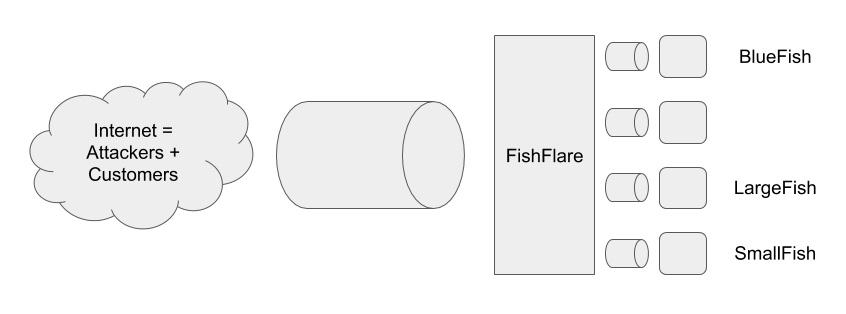
\includegraphics[scale=0.5]{FishFlare}

In order to provide protection against such large scale attacks, a new company
\texttt{FishFlare} provides a DoS mitigation service to its customers. This is
how it works: a customer, \texttt{BlueFish}, points the DNS entry for
\texttt{bluefish.com} to \texttt{FishFlare}'s servers, and tells
\texttt{FishFlare} about the real IP address that host \texttt{bluefish.com}'s
content. This way, \texttt{FishFlare} sits between the customers of
\texttt{BlueFish} and actual servers hosting content for \texttt{bluefish.com}
(see the figure above).\footnote{Note that this still leaves
\texttt{BlueFish} vulnerable, since anyone who can figure out the real IP
address can launch DDoS directly against \texttt{BlueFish} without going through
\texttt{FishFlare}. This DNS based technique is merely one solution that fits
small-scale businesses. The actual techniques used by large corporations are
slightly more involved and require a bit nuanced knowledge of how the Internet
routing works (specifically BGP), and context (whether a victim can seek help
from its ISP in some filtering). You may learn about this more in a networking
class; we ignore the details here to get the high-level idea across.}

The hope is once \texttt{FishFlare} acquires enough customers, it can also
acquire large enough bandwidth to withstand very large DDoS attacks with the
cost amortized over a large number of customers. Since all the traffic passes
through \texttt{FishFlare}, it can \emph{scrub}-away the bogus traffic and only
send cleaned-up traffic to actual \texttt{BlueFish} infrastructure.

How can \texttt{FishFlare} cleanup the \texttt{memcached}-based attack on the 
website of one of its customers? In no more than 2 sentences, describe an 
efficient strategy that works at line rate and is effective (\emph{i.e.}\ very
few, if any, false positives or false negatives).


\textfield{Q4P4}{3cm}{
%Your solution to Q4 part 4 here
Block all inbound traffics except established TCP connections or packets that try to establish a TCP connection.
}

\end{parts}



\newpage
\titledquestion{Reconnaissance Attacks}[15]

\def\patsy{$\mathcal{P}$\xspace}
\def\control{$\mathcal{A}$\xspace}
\def\victim{$\mathcal{V}$\xspace}

The IP packet header contains a 16-bit ID field that is used for assembling
packet fragments.\footnote{
	For now, don't worry about how such fragments work.
	For this problem, we only care that this field exists and
	how hosts set it in the packets they send.
}
The protocol standard states that the ID field should differ between
different packets sent by a source to a given destination.\footnote{
	Clearly, if a host sends more than $2^{16}$ packets,
	the field will necessarily
	repeat.  That consideration doesn't matter for this problem, either!
}
A common method that hosts use to implement the
ID field is to maintain a single counter that the host increments by one
for every packet it sends, regardless of to which destination it
sends it. The host sets the ID field in each packet it sends to
the current value of the counter.
Since with this implementation the host uses a single counter for all of
its connections, we say that
the host implements a \emph{global ID field}.

\begin{parts}
\part Suppose a host \patsy implements a global ID field. Suppose further that
\patsy responds to ICMP ping requests. You control some other host \control.
How can you test if \patsy sent a packet to anyone (other than \control) within
a certain one minute window? Can you use that same method to test if \patsy received
a packet from anyone within a certain one minute window? You are allowed to send your own packets to
\patsy.

\textfield{Q5P1}{3cm}{
%Your solution to Q5 part 1 here
Let \control send a ICMP ping request to host \patsy before and after this one minute window. Check the ID field in response packets. If they're differed by 1, \patsy didn't send packet to anyone else. Otherwise \patsy did sent packets to someone.

This method cannot test whether \patsy receive a packet from anyone.
}


\part Your goal now is to test whether a victim host \victim is running a
server that accepts connections to TCP port $n$ (that is, test if \victim is
listening on TCP port $n$).  You wish to hide the identity of your machine
\control. Hence, \control cannot directly send a packet to \victim, unless that
packet contains a spoofed source IP address.  Explain how to use \patsy to do this, assuming that 
\patsy is quiescent during this test. If \patsy is not quiescent during the test, will this method still work? 
Why or why not?

\textsc{Hint}: recall the following facts about TCP.
\begin{itemize}
\item A host that receives a SYN packet to an open port $n$ sends back a
  SYN/ACK response to the source address.
\item A host that receives a SYN packet to a closed port $n$ sends back a RST
  packet to the source address.
\item A host that receives a SYN/ACK packet that it is not expecting sends back
  a RST packet to the source address.
\item A host that receives a RST packet sends back no response.
\end{itemize}


\textfield{Q5P2}{5cm}{
%Your solution to Q5 part 2 here
Send a SYN packet to \victim with a spoofed source IP address(source address is \patsy's). Then check whether \patsy send a packet using the method mentioned previously. If \patsy did send, \victim is listening on TCP port $n$. Otherwise, it didn't. This method works because \victim will send a SYN/ACK packet to \patsy, and \patsy will respond with a RST packet.

If \patsy is not quiescent during the test, this method doesn't work anymore. Because we cannot determine whether \patsy send a packet to \victim or someone else.

}


\part How would you change \patsy to stop these attacks? You are not allowed to
modify the TCP/IP protocol or the services running on \patsy. You may only
modify the \emph{implementation} of TCP/IP on \patsy. 


\textfield{Q5P3}{5cm}{
%Your solution to Q5 part 2 here
Let \patsy maintain a counter for each pair of source address and destination address.
}

\end{parts}

\end{questions}
\end{Form}
\end{document}
